% Options for packages loaded elsewhere
\PassOptionsToPackage{unicode}{hyperref}
\PassOptionsToPackage{hyphens}{url}
\documentclass[
]{article}
\usepackage{xcolor}
\usepackage[margin=1in]{geometry}
\usepackage{amsmath,amssymb}
\setcounter{secnumdepth}{5}
\usepackage{iftex}
\ifPDFTeX
  \usepackage[T1]{fontenc}
  \usepackage[utf8]{inputenc}
  \usepackage{textcomp} % provide euro and other symbols
\else % if luatex or xetex
  \usepackage{unicode-math} % this also loads fontspec
  \defaultfontfeatures{Scale=MatchLowercase}
  \defaultfontfeatures[\rmfamily]{Ligatures=TeX,Scale=1}
\fi
\usepackage{lmodern}
\ifPDFTeX\else
  % xetex/luatex font selection
\fi
% Use upquote if available, for straight quotes in verbatim environments
\IfFileExists{upquote.sty}{\usepackage{upquote}}{}
\IfFileExists{microtype.sty}{% use microtype if available
  \usepackage[]{microtype}
  \UseMicrotypeSet[protrusion]{basicmath} % disable protrusion for tt fonts
}{}
\makeatletter
\@ifundefined{KOMAClassName}{% if non-KOMA class
  \IfFileExists{parskip.sty}{%
    \usepackage{parskip}
  }{% else
    \setlength{\parindent}{0pt}
    \setlength{\parskip}{6pt plus 2pt minus 1pt}}
}{% if KOMA class
  \KOMAoptions{parskip=half}}
\makeatother
\usepackage{color}
\usepackage{fancyvrb}
\newcommand{\VerbBar}{|}
\newcommand{\VERB}{\Verb[commandchars=\\\{\}]}
\DefineVerbatimEnvironment{Highlighting}{Verbatim}{commandchars=\\\{\}}
% Add ',fontsize=\small' for more characters per line
\usepackage{framed}
\definecolor{shadecolor}{RGB}{248,248,248}
\newenvironment{Shaded}{\begin{snugshade}}{\end{snugshade}}
\newcommand{\AlertTok}[1]{\textcolor[rgb]{0.94,0.16,0.16}{#1}}
\newcommand{\AnnotationTok}[1]{\textcolor[rgb]{0.56,0.35,0.01}{\textbf{\textit{#1}}}}
\newcommand{\AttributeTok}[1]{\textcolor[rgb]{0.13,0.29,0.53}{#1}}
\newcommand{\BaseNTok}[1]{\textcolor[rgb]{0.00,0.00,0.81}{#1}}
\newcommand{\BuiltInTok}[1]{#1}
\newcommand{\CharTok}[1]{\textcolor[rgb]{0.31,0.60,0.02}{#1}}
\newcommand{\CommentTok}[1]{\textcolor[rgb]{0.56,0.35,0.01}{\textit{#1}}}
\newcommand{\CommentVarTok}[1]{\textcolor[rgb]{0.56,0.35,0.01}{\textbf{\textit{#1}}}}
\newcommand{\ConstantTok}[1]{\textcolor[rgb]{0.56,0.35,0.01}{#1}}
\newcommand{\ControlFlowTok}[1]{\textcolor[rgb]{0.13,0.29,0.53}{\textbf{#1}}}
\newcommand{\DataTypeTok}[1]{\textcolor[rgb]{0.13,0.29,0.53}{#1}}
\newcommand{\DecValTok}[1]{\textcolor[rgb]{0.00,0.00,0.81}{#1}}
\newcommand{\DocumentationTok}[1]{\textcolor[rgb]{0.56,0.35,0.01}{\textbf{\textit{#1}}}}
\newcommand{\ErrorTok}[1]{\textcolor[rgb]{0.64,0.00,0.00}{\textbf{#1}}}
\newcommand{\ExtensionTok}[1]{#1}
\newcommand{\FloatTok}[1]{\textcolor[rgb]{0.00,0.00,0.81}{#1}}
\newcommand{\FunctionTok}[1]{\textcolor[rgb]{0.13,0.29,0.53}{\textbf{#1}}}
\newcommand{\ImportTok}[1]{#1}
\newcommand{\InformationTok}[1]{\textcolor[rgb]{0.56,0.35,0.01}{\textbf{\textit{#1}}}}
\newcommand{\KeywordTok}[1]{\textcolor[rgb]{0.13,0.29,0.53}{\textbf{#1}}}
\newcommand{\NormalTok}[1]{#1}
\newcommand{\OperatorTok}[1]{\textcolor[rgb]{0.81,0.36,0.00}{\textbf{#1}}}
\newcommand{\OtherTok}[1]{\textcolor[rgb]{0.56,0.35,0.01}{#1}}
\newcommand{\PreprocessorTok}[1]{\textcolor[rgb]{0.56,0.35,0.01}{\textit{#1}}}
\newcommand{\RegionMarkerTok}[1]{#1}
\newcommand{\SpecialCharTok}[1]{\textcolor[rgb]{0.81,0.36,0.00}{\textbf{#1}}}
\newcommand{\SpecialStringTok}[1]{\textcolor[rgb]{0.31,0.60,0.02}{#1}}
\newcommand{\StringTok}[1]{\textcolor[rgb]{0.31,0.60,0.02}{#1}}
\newcommand{\VariableTok}[1]{\textcolor[rgb]{0.00,0.00,0.00}{#1}}
\newcommand{\VerbatimStringTok}[1]{\textcolor[rgb]{0.31,0.60,0.02}{#1}}
\newcommand{\WarningTok}[1]{\textcolor[rgb]{0.56,0.35,0.01}{\textbf{\textit{#1}}}}
\usepackage{graphicx}
\makeatletter
\newsavebox\pandoc@box
\newcommand*\pandocbounded[1]{% scales image to fit in text height/width
  \sbox\pandoc@box{#1}%
  \Gscale@div\@tempa{\textheight}{\dimexpr\ht\pandoc@box+\dp\pandoc@box\relax}%
  \Gscale@div\@tempb{\linewidth}{\wd\pandoc@box}%
  \ifdim\@tempb\p@<\@tempa\p@\let\@tempa\@tempb\fi% select the smaller of both
  \ifdim\@tempa\p@<\p@\scalebox{\@tempa}{\usebox\pandoc@box}%
  \else\usebox{\pandoc@box}%
  \fi%
}
% Set default figure placement to htbp
\def\fps@figure{htbp}
\makeatother
\setlength{\emergencystretch}{3em} % prevent overfull lines
\providecommand{\tightlist}{%
  \setlength{\itemsep}{0pt}\setlength{\parskip}{0pt}}
\usepackage[]{natbib}
\bibliographystyle{plainnat}
\usepackage{bookmark}
\IfFileExists{xurl.sty}{\usepackage{xurl}}{} % add URL line breaks if available
\urlstyle{same}
\hypersetup{
  pdftitle={HW 02 - Airbnb listings in Edinburgh},
  pdfauthor={Tina Huynh},
  hidelinks,
  pdfcreator={LaTeX via pandoc}}

\title{HW 02 - Airbnb listings in Edinburgh}
\author{Tina Huynh}
\date{}

\begin{document}
\maketitle

{
\setcounter{tocdepth}{2}
\tableofcontents
}
\begin{figure}
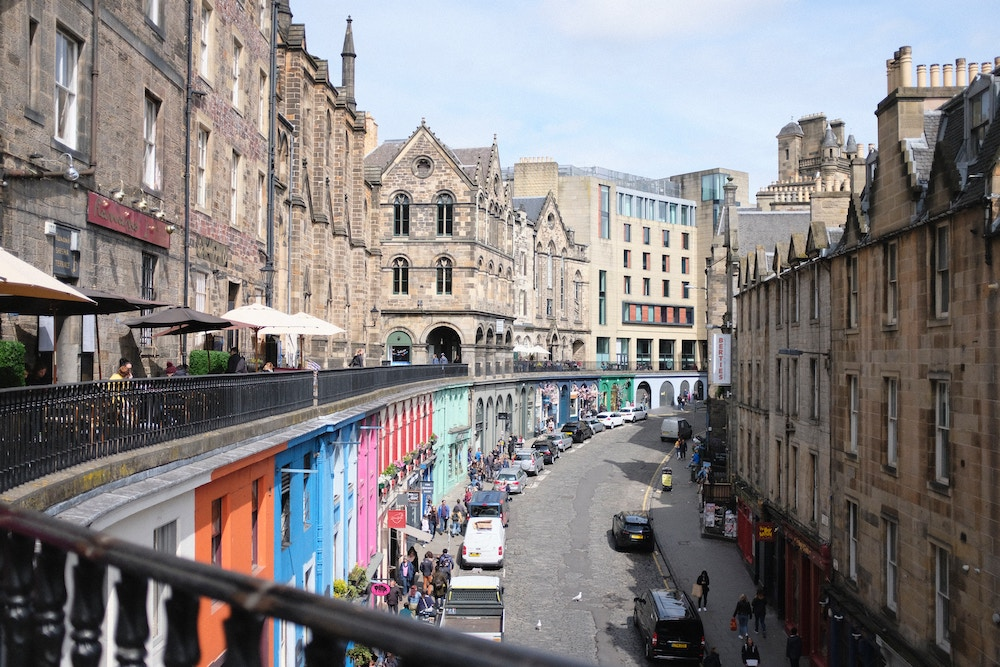
\includegraphics[width=0.8\linewidth]{img/madeleine-kohler-90Qn643Pq9c-unsplash} \caption{Photo by Madeleine Kohler on Unsplash}\label{fig:photo}
\end{figure}

Once upon a time, people traveled all over the world, and some stayed in
hotels and others chose to stay in other people's houses that they
booked through Airbnb. Recent developments in Edinburgh regarding the
growth of Airbnb and its impact on the housing market means a better
understanding of the Airbnb listings is needed. Using data provided by
Airbnb, we can explore how Airbnb availability and prices vary by
neighbourhood.

\section{Getting started}\label{getting-started}

\begin{marginnote}
\textbf{IMPORTANT:} If there is no GitHub repo created for you for this
assignment, it means I didn't have your GitHub username as of when I
assigned the homework. Please let me know your GitHub username asap, and
I can create your repo.
\end{marginnote}

Go to the course GitHub organization and locate your homework repo,
which should be named \texttt{hw-02-airbnb-edi-YOUR\_GITHUB\_USERNAME}.
Grab the URL of the repo, and clone it in RStudio. First, open the R
Markdown document \texttt{hw-02.Rmd} and Knit it. Make sure it compiles
without errors. The output will be in the file markdown \texttt{.md}
file with the same name.

\subsection{Warm up}\label{warm-up}

Before we introduce the data, let's warm up with some simple exercises.

\begin{itemize}
\tightlist
\item
  Update the YAML, changing the author name to your name, and
  \textbf{knit} the document.
\item
  Commit your changes with a meaningful commit message.
\item
  Push your changes to GitHub.
\item
  Go to your repo on GitHub and confirm that your changes are visible in
  your Rmd \textbf{and} md files. If anything is missing, commit and
  push again.
\end{itemize}

\subsection{Packages}\label{packages}

We'll use the \textbf{tidyverse} package for much of the data wrangling
and visualization and the data lives in the \textbf{dsbox} package.
These packages are already installed for you. You can load them by
running the following in your Console:

\begin{Shaded}
\begin{Highlighting}[]
\FunctionTok{install.packages}\NormalTok{(}\StringTok{"devtools"}\NormalTok{)}
\NormalTok{devtools}\SpecialCharTok{::}\FunctionTok{install\_github}\NormalTok{(}\StringTok{"tidyverse/dsbox"}\NormalTok{)}
\FunctionTok{library}\NormalTok{(tidyverse)}
\FunctionTok{library}\NormalTok{(dsbox)}
\end{Highlighting}
\end{Shaded}

\subsection{Data}\label{data}

The data can be found in the \textbf{dsbox} package, and it's called
\texttt{edibnb}. Since the dataset is distributed with the package, we
don't need to load it separately; it becomes available to us when we
load the package.

You can view the dataset as a spreadsheet using the \texttt{View()}
function. Note that you should not put this function in your R Markdown
document, but instead type it directly in the Console, as it pops open a
new window (and the concept of popping open a window in a static
document doesn't really make sense\ldots). When you run this in the
console, you'll see the following \textbf{data viewer} window pop up.

\begin{Shaded}
\begin{Highlighting}[]
\FunctionTok{View}\NormalTok{(edibnb)}
\end{Highlighting}
\end{Shaded}

You can find out more about the dataset by inspecting its documentation,
which you can access by running \texttt{?edibnb} in the Console or using
the Help menu in RStudio to search for \texttt{edibnb}.

\section{Exercises}\label{exercises}

\begin{marginnote}
\textbf{Hint:} The Markdown Quick Reference sheet has an example of
inline R code that might be helpful. You can access it from the Help
menu in RStudio.
\end{marginnote}

\begin{enumerate}
\def\labelenumi{\arabic{enumi}.}
\item
  How many observations (rows) does the dataset have? 13245 entities in
  total
\item
  Run \texttt{View(edibnb)} in your Console to view the data in the data
  viewer. What does each row in the dataset represent?\\
  \textbf{Each data row represents a listing for an Airbnb rental in
  Edinburgh.}
\end{enumerate}

🧶 ✅ ⬆️ \emph{Knit,} \emph{commit, and push your changes to GitHub with
an appropriate commit message. Make sure to commit and push all changed
files so that your Git pane is cleared up afterwards.}

We can get a list of the variables in the data frame using the
\texttt{names()} function.

\begin{Shaded}
\begin{Highlighting}[]
\FunctionTok{names}\NormalTok{(edibnb)}
\end{Highlighting}
\end{Shaded}

\begin{verbatim}
##  [1] "id"                   "price"                "neighbourhood"       
##  [4] "accommodates"         "bathrooms"            "bedrooms"            
##  [7] "beds"                 "review_scores_rating" "number_of_reviews"   
## [10] "listing_url"
\end{verbatim}

You can find descriptions of each of the variables in the help file for
the dataset, which you can access by running \texttt{?edibnb} in your
Console.

\begin{marginnote}
\textbf{Note:} The plot will give a warning about some observations with
non-finite values for price being removed. Don't worry about the
warning, it simply means that 199 listings in the data didn't have
prices available, so they can't be plotted.
\end{marginnote}

\begin{enumerate}
\def\labelenumi{\arabic{enumi}.}
\tightlist
\item
  Create a faceted histogram where each facet represents a neighbourhood
  and displays the distribution of Airbnb prices in that neighbourhood.
  Think critically about whether it makes more sense to stack the facets
  on top of each other in a column, lay them out in a row, or wrap them
  around. Along with your visualization, include your reasoning for the
  layout you chose for your facets.
\end{enumerate}

\begin{Shaded}
\begin{Highlighting}[]
\FunctionTok{ggplot}\NormalTok{(edibnb, }\FunctionTok{aes}\NormalTok{(}\AttributeTok{x =}\NormalTok{ price)) }\SpecialCharTok{+}
  \FunctionTok{geom\_histogram}\NormalTok{(}\FunctionTok{aes}\NormalTok{(}\AttributeTok{y =} \FunctionTok{after\_stat}\NormalTok{(density)), }\AttributeTok{bins =} \DecValTok{25}\NormalTok{, }\AttributeTok{boundary =} \DecValTok{10}\NormalTok{, }\AttributeTok{closed =} \StringTok{"left"}\NormalTok{) }\SpecialCharTok{+}
  \FunctionTok{coord\_cartesian}\NormalTok{(}\AttributeTok{xlim =} \FunctionTok{c}\NormalTok{(}\DecValTok{0}\NormalTok{, }\FunctionTok{quantile}\NormalTok{(edibnb}\SpecialCharTok{$}\NormalTok{price, }\FloatTok{0.99}\NormalTok{, }\AttributeTok{na.rm =} \ConstantTok{TRUE}\NormalTok{))) }\SpecialCharTok{+}
  \FunctionTok{facet\_wrap}\NormalTok{(}\SpecialCharTok{\textasciitilde{}}\NormalTok{ neighbourhood, }\AttributeTok{ncol =} \DecValTok{5}\NormalTok{) }\SpecialCharTok{+}
  \FunctionTok{labs}\NormalTok{(}
    \AttributeTok{title =} \StringTok{"Edinburgh Airbnb Price Distributions by neighbourhood"}\NormalTok{,}
    \AttributeTok{subtitle =} \StringTok{"Density{-}scaled histograms; x{-}axis capped at the 99th percentile"}\NormalTok{,}
    \AttributeTok{x =} \StringTok{"Price (GBP)"}\NormalTok{,}
    \AttributeTok{y =} \StringTok{"Density"}\NormalTok{,}
    \AttributeTok{caption =} \StringTok{"Source: dsbox::edibnb (Inside Airbnb / Kaggle)"}
\NormalTok{  ) }\SpecialCharTok{+}
  \FunctionTok{theme\_minimal}\NormalTok{(}\AttributeTok{base\_size =} \DecValTok{13}\NormalTok{) }\SpecialCharTok{+}
  \FunctionTok{theme}\NormalTok{(}
    \AttributeTok{strip.text =} \FunctionTok{element\_text}\NormalTok{(}\AttributeTok{size =} \DecValTok{10}\NormalTok{),}
    \AttributeTok{panel.grid.minor =} \FunctionTok{element\_blank}\NormalTok{(),}
    \AttributeTok{axis.text =} \FunctionTok{element\_text}\NormalTok{(}\AttributeTok{size =} \DecValTok{6}\NormalTok{),}
    \AttributeTok{plot.margin =} \FunctionTok{unit}\NormalTok{(}\FunctionTok{c}\NormalTok{(}\FloatTok{0.5}\NormalTok{, }\FloatTok{0.25}\NormalTok{, }\FloatTok{0.5}\NormalTok{, }\FloatTok{0.25}\NormalTok{), }\StringTok{"cm"}\NormalTok{)}
\NormalTok{  )}
\end{Highlighting}
\end{Shaded}

\begin{verbatim}
## Warning: Removed 199 rows containing non-finite outside the scale range
## (`stat_bin()`).
\end{verbatim}

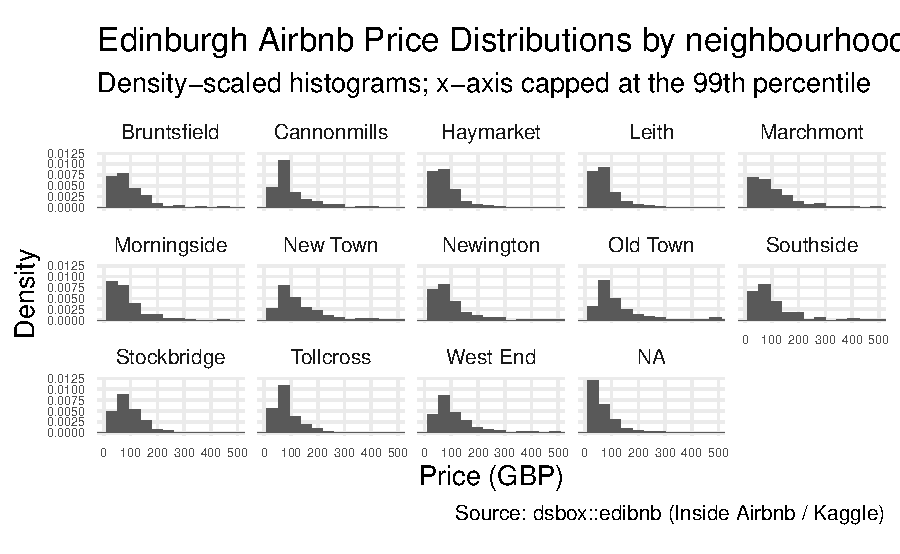
\includegraphics[width=0.8\linewidth]{hw-02-airbnb-edi_files/figure-latex/unnamed-chunk-6-1}

Let's de-construct this code:

\begin{itemize}
\tightlist
\item
  \texttt{ggplot()} is the function we are using to build our plot, in
  layers.
\item
  In the first layer we always define the data frame as the first
  argument. Then, we define the mappings between the variables in the
  dataset and the \textbf{aes}thetics of the plot (e.g.~x and y
  coordinates, colours, etc.).
\item
  In the next layer we represent the data with \textbf{geom}etric
  shapes, in this case with a histogram. You should decide what makes a
  reasonable bin width for the histogram by trying out a few options.
\item
  In the final layer we facet the data by neighbourhood.
\end{itemize}

I chose to use \texttt{facet\_wrap()} with 5 columns because:

\begin{enumerate}
\def\labelenumi{\arabic{enumi}.}
\item
  Edinburgh has multiple neighborhoods, and wrapping them allows for
  better use of the horizontal space than a single column or row. This
  way, we can see more neighborhoods at once without excessive
  scrolling.
\item
  With 5 columns, each facet is still large enough to see the
  distribution clearly and not too compressed.
\item
  This layout makes it easier to compare neighborhoods at a glance than
  stacking them in a column. Therefore, it is more efficient for visual
  comparison.
\item
  The wrapped layout provides a good balance between detail and overall
  comparison view because it avoids excessive white space that would
  occur with too few columns.
\end{enumerate}

🧶 ✅ ⬆️ Knit, \emph{commit, and push your changes to GitHub with an
appropriate commit message. Make sure to commit and push all changed
files so that your Git pane is cleared up afterwards.}

\begin{enumerate}
\def\labelenumi{\arabic{enumi}.}
\setcounter{enumi}{3}
\tightlist
\item
  Use a single pipeline to identity the neighbourhoods with the top five
  median listing prices. Then, in another pipeline filter the data for
  these five neighbourhoods and make ridge plots of the distributions of
  listing prices in these five neighbourhoods. In a third pipeline
  calculate the minimum, mean, median, standard deviation, IQR, and
  maximum listing price in each of these neighbourhoods. Use the
  visualization and the summary statistics to describe the distribution
  of listing prices in the neighbourhoods. (Your answer will include
  three pipelines, one of which ends in a visualization, and a
  narrative.)
\end{enumerate}

\begin{Shaded}
\begin{Highlighting}[]
\NormalTok{top5\_neighbourhoods }\OtherTok{\textless{}{-}}\NormalTok{ edibnb }\SpecialCharTok{\%\textgreater{}\%}
  \FunctionTok{filter}\NormalTok{(}\SpecialCharTok{!}\FunctionTok{is.na}\NormalTok{(price), price }\SpecialCharTok{\textgreater{}} \DecValTok{0}\NormalTok{, }\SpecialCharTok{!}\FunctionTok{is.na}\NormalTok{(neighbourhood)) }\SpecialCharTok{\%\textgreater{}\%}
  \FunctionTok{group\_by}\NormalTok{(neighbourhood) }\SpecialCharTok{\%\textgreater{}\%}
  \FunctionTok{summarize}\NormalTok{(}\AttributeTok{median\_price =} \FunctionTok{median}\NormalTok{(price, }\AttributeTok{na.rm =} \ConstantTok{TRUE}\NormalTok{)) }\SpecialCharTok{\%\textgreater{}\%}
  \FunctionTok{arrange}\NormalTok{(}\FunctionTok{desc}\NormalTok{(median\_price)) }\SpecialCharTok{\%\textgreater{}\%}
  \FunctionTok{slice\_head}\NormalTok{(}\AttributeTok{n =} \DecValTok{5}\NormalTok{)}

\NormalTok{top5\_neighbourhoods}
\end{Highlighting}
\end{Shaded}

\begin{verbatim}
## # A tibble: 5 x 2
##   neighbourhood median_price
##   <chr>                <dbl>
## 1 New Town               100
## 2 Old Town                90
## 3 West End                90
## 4 Stockbridge             85
## 5 Bruntsfield             80
\end{verbatim}

\begin{Shaded}
\begin{Highlighting}[]
\FunctionTok{library}\NormalTok{(ggridges)}

\NormalTok{edibnb }\SpecialCharTok{\%\textgreater{}\%}
  \FunctionTok{filter}\NormalTok{(}\SpecialCharTok{!}\FunctionTok{is.na}\NormalTok{(price), price }\SpecialCharTok{\textgreater{}} \DecValTok{0}\NormalTok{, neighbourhood }\SpecialCharTok{\%in\%}\NormalTok{ top5\_neighbourhoods}\SpecialCharTok{$}\NormalTok{neighbourhood) }\SpecialCharTok{\%\textgreater{}\%}
  \FunctionTok{ggplot}\NormalTok{(}\FunctionTok{aes}\NormalTok{(}\AttributeTok{x =}\NormalTok{ price, }\AttributeTok{y =}\NormalTok{ neighbourhood, }\AttributeTok{fill =}\NormalTok{ neighbourhood)) }\SpecialCharTok{+}
  \FunctionTok{geom\_density\_ridges}\NormalTok{(}\AttributeTok{alpha =} \FloatTok{0.6}\NormalTok{, }\AttributeTok{scale =} \FloatTok{1.2}\NormalTok{, }\AttributeTok{rel\_min\_height =} \FloatTok{0.01}\NormalTok{) }\SpecialCharTok{+}
  \FunctionTok{coord\_cartesian}\NormalTok{(}\AttributeTok{xlim =} \FunctionTok{c}\NormalTok{(}\DecValTok{0}\NormalTok{, }\FunctionTok{quantile}\NormalTok{(dsbox}\SpecialCharTok{::}\NormalTok{edibnb}\SpecialCharTok{$}\NormalTok{price, }\FloatTok{0.99}\NormalTok{, }\AttributeTok{na.rm =} \ConstantTok{TRUE}\NormalTok{))) }\SpecialCharTok{+}
  \FunctionTok{labs}\NormalTok{(}
    \AttributeTok{title =} \StringTok{"Price Distributions of Top 5 Most Expensive neighbourhoods in Edinburgh"}\NormalTok{,}
    \AttributeTok{x =} \StringTok{"Listing Price (GBP)"}\NormalTok{,}
    \AttributeTok{y =} \StringTok{"neighbourhood"}
\NormalTok{  ) }\SpecialCharTok{+}
  \FunctionTok{theme\_minimal}\NormalTok{(}\AttributeTok{base\_size =} \DecValTok{12}\NormalTok{) }\SpecialCharTok{+}
  \FunctionTok{theme}\NormalTok{(}\AttributeTok{legend.position =} \StringTok{"none"}\NormalTok{)}
\end{Highlighting}
\end{Shaded}

\begin{verbatim}
## Picking joint bandwidth of 13.8
\end{verbatim}

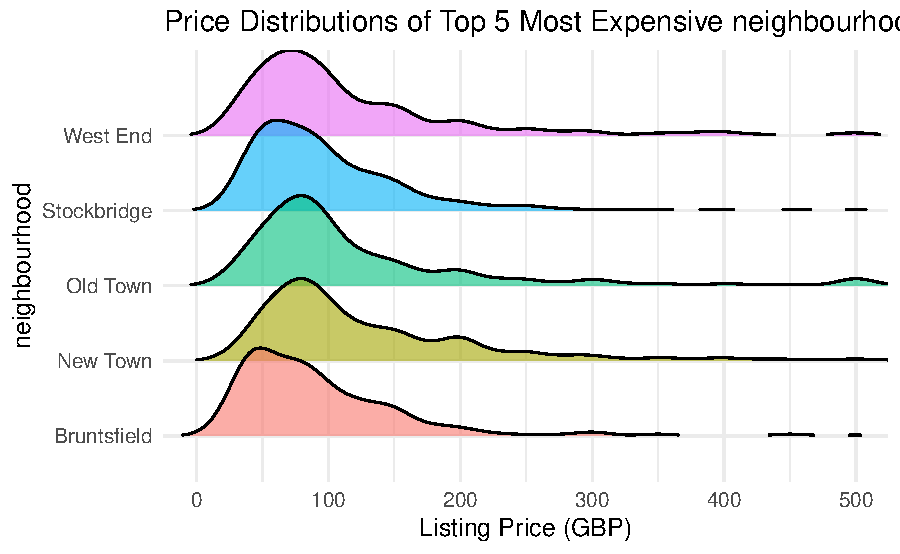
\includegraphics[width=0.8\linewidth]{hw-02-airbnb-edi_files/figure-latex/unnamed-chunk-8-1}

\begin{Shaded}
\begin{Highlighting}[]
\NormalTok{summary\_stats }\OtherTok{\textless{}{-}}\NormalTok{ edibnb }\SpecialCharTok{\%\textgreater{}\%}
  \FunctionTok{filter}\NormalTok{(}\SpecialCharTok{!}\FunctionTok{is.na}\NormalTok{(price), price }\SpecialCharTok{\textgreater{}} \DecValTok{0}\NormalTok{, neighbourhood }\SpecialCharTok{\%in\%}\NormalTok{ top5\_neighbourhoods}\SpecialCharTok{$}\NormalTok{neighbourhood) }\SpecialCharTok{\%\textgreater{}\%}
  \FunctionTok{group\_by}\NormalTok{(neighbourhood) }\SpecialCharTok{\%\textgreater{}\%}
  \FunctionTok{summarize}\NormalTok{(}
    \AttributeTok{min\_price =} \FunctionTok{min}\NormalTok{(price, }\AttributeTok{na.rm =} \ConstantTok{TRUE}\NormalTok{),}
    \AttributeTok{mean\_price =} \FunctionTok{mean}\NormalTok{(price, }\AttributeTok{na.rm =} \ConstantTok{TRUE}\NormalTok{),}
    \AttributeTok{median\_price =} \FunctionTok{median}\NormalTok{(price, }\AttributeTok{na.rm =} \ConstantTok{TRUE}\NormalTok{),}
    \AttributeTok{sd\_price =} \FunctionTok{sd}\NormalTok{(price, }\AttributeTok{na.rm =} \ConstantTok{TRUE}\NormalTok{),}
    \AttributeTok{iqr\_price =} \FunctionTok{IQR}\NormalTok{(price, }\AttributeTok{na.rm =} \ConstantTok{TRUE}\NormalTok{),}
    \AttributeTok{max\_price =} \FunctionTok{max}\NormalTok{(price, }\AttributeTok{na.rm =} \ConstantTok{TRUE}\NormalTok{)}
\NormalTok{  )}

\NormalTok{summary\_stats}
\end{Highlighting}
\end{Shaded}

\begin{verbatim}
## # A tibble: 5 x 7
##   neighbourhood min_price mean_price median_price sd_price iqr_price max_price
##   <chr>             <dbl>      <dbl>        <dbl>    <dbl>     <dbl>     <dbl>
## 1 Bruntsfield          10       99.4           80     90.2      72.5       900
## 2 New Town             12      136.           100    109.       86.5       999
## 3 Old Town             15      128.            90    110.       76         999
## 4 Stockbridge          21      104.            85     77.6      66         750
## 5 West End             19      116.            90     93.3      80         999
\end{verbatim}

The price distributions in all five neighborhoods demonstrate pronounced
positive skewness, characterized by a concentration of listings at
moderate price points with an extended tail toward higher values. This
asymmetry suggests a market structure where most properties maintain
accessible pricing while a select subset commands premium rates.

New Town, with the highest median price (£100), exhibits the most
pronounced variance (standard deviation of £108.59), indicating
considerable price stratification within this historically significant
district. This variability likely reflects the neighborhood's diverse
property portfolio, ranging from modest apartments to luxury Georgian
residences. The substantial interquartile range (£86.50) further
confirms this price diversity, suggesting potential investment
opportunities across various market segments.

Stockbridge and West End complete the top five neighborhoods, displaying
intermediate pricing patterns. Notably, Stockbridge exhibits the lowest
standard deviation (£77.57) among these premium areas, potentially
signifying a more uniform housing stock. The median price (£85) and
interquartile range (£76) suggest a balanced market, appealing to both
mid-range and higher-end renters.

Old Town, despite its status as a primary tourist destination, presents
a slightly lower median price (£90) compared to New Town, while
maintaining comparable variability (standard deviation of £109.57). This
pattern may reflect the neighborhood's mixed accommodation offerings,
from heritage buildings to more contemporary developments. The area's
tourism appeal evidently supports elevated price points, with maximum
values reaching £999.

Bruntsfield demonstrates a more concentrated price distribution
(standard deviation of £90.17) relative to its median (£80), suggesting
greater homogeneity in property types and quality within this
neighborhood. This characteristic could indicate a more stable,
predictable market with potentially lower investment risk.

The minimum listing prices remain relatively consistent across all five
neighborhoods (ranging from £10-£21), indicating that even in
Edinburgh's most exclusive districts, budget accommodation options
exist. This accessibility at the lower end contrasts sharply with the
maximum values, which reach £999 in multiple neighborhoods, highlighting
significant market segmentation.

These pricing patterns reflect Edinburgh's complex residential
landscape, where historical significance, architectural heritage, and
proximity to cultural attractions interact to create distinctive
neighborhood value propositions. The data suggests that New Town and Old
Town command premium pricing due to their central location and
historical importance, while areas like Bruntsfield may offer more
consistent pricing expectations for both investors and visitors seeking
accommodation.

\begin{enumerate}
\def\labelenumi{\arabic{enumi}.}
\setcounter{enumi}{4}
\tightlist
\item
  Create a visualization that will help you compare the distribution of
  review scores (\texttt{review\_scores\_rating}) across neighborhoods.
  You get to decide what type of visualization to create and there is
  more than one correct answer! In your answer, include a brief
  interpretation of how Airbnb guests rate properties in general and how
  the neighborhoods compare to each other in terms of their ratings.
\end{enumerate}

\begin{Shaded}
\begin{Highlighting}[]
\FunctionTok{ggplot}\NormalTok{(edibnb }\SpecialCharTok{\%\textgreater{}\%}
  \FunctionTok{filter}\NormalTok{(}\SpecialCharTok{!}\FunctionTok{is.na}\NormalTok{(review\_scores\_rating), }\SpecialCharTok{!}\FunctionTok{is.na}\NormalTok{(neighbourhood)) }\SpecialCharTok{\%\textgreater{}\%}
  \FunctionTok{mutate}\NormalTok{(}
    \AttributeTok{neighbourhood =} \FunctionTok{fct\_reorder}\NormalTok{(neighbourhood, review\_scores\_rating, }\AttributeTok{.fun =}\NormalTok{ median, }\AttributeTok{.na\_rm =} \ConstantTok{TRUE}\NormalTok{)}
\NormalTok{  ), }\FunctionTok{aes}\NormalTok{(}\AttributeTok{x =}\NormalTok{ neighbourhood, }\AttributeTok{y =}\NormalTok{ review\_scores\_rating)) }\SpecialCharTok{+}
  \FunctionTok{geom\_boxplot}\NormalTok{(}\AttributeTok{fill =} \StringTok{"steelblue"}\NormalTok{, }\AttributeTok{alpha =} \FloatTok{0.6}\NormalTok{, }\AttributeTok{outlier.alpha =} \FloatTok{0.3}\NormalTok{) }\SpecialCharTok{+}
  \FunctionTok{coord\_flip}\NormalTok{() }\SpecialCharTok{+}
  \FunctionTok{labs}\NormalTok{(}
    \AttributeTok{title =} \StringTok{"Distribution of Airbnb Review Scores by neighbourhood in Edinburgh"}\NormalTok{,}
    \AttributeTok{x =} \StringTok{"neighbourhood"}\NormalTok{,}
\NormalTok{    y }\OtherTok{\textless{}{-}} \StringTok{"Review Score (0{-}100)"}
\NormalTok{  ) }\SpecialCharTok{+}
  \FunctionTok{theme\_minimal}\NormalTok{(}\AttributeTok{base\_size =} \DecValTok{12}\NormalTok{) }\SpecialCharTok{+}
  \FunctionTok{theme}\NormalTok{(}
    \AttributeTok{panel.grid.minor =} \FunctionTok{element\_blank}\NormalTok{(),}
    \AttributeTok{axis.text.y =} \FunctionTok{element\_text}\NormalTok{(}\AttributeTok{size =} \DecValTok{9}\NormalTok{)}
\NormalTok{  )}
\end{Highlighting}
\end{Shaded}

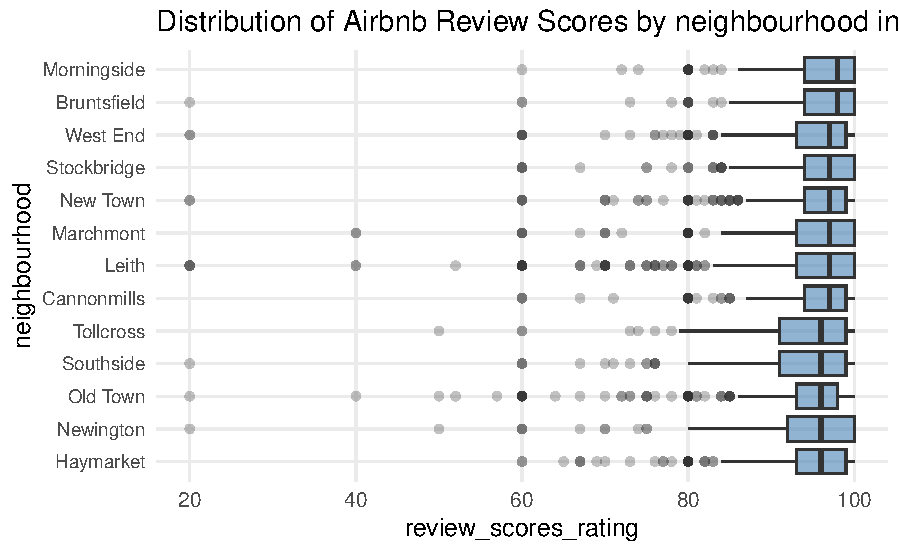
\includegraphics[width=0.8\linewidth]{hw-02-airbnb-edi_files/figure-latex/unnamed-chunk-10-1}

The visualization of review score distributions reveals nuanced patterns
in guest satisfaction across Edinburgh's diverse neighborhoods.
Examination of the boxplots indicates a predominantly positive guest
experience throughout the city, with most neighborhoods achieving median
ratings exceeding 90 on the 100-point scale. This high baseline suggests
Edinburgh's Airbnb market generally delivers satisfactory accommodations
regardless of location.

Notable in this analysis is the inverse relationship between
accommodation cost and guest satisfaction. The neighborhoods commanding
premium pricing---particularly New Town and West End---paradoxically
rank lower in guest satisfaction than more moderately priced areas. This
phenomenon may reflect guests' value expectations; higher-priced
accommodations potentially trigger heightened expectations that prove
challenging to fulfill consistently. Conversely, neighborhoods like
Stockbridge, South Side, and Leith, which offer more moderate pricing,
achieve superior satisfaction ratings, possibly because they exceed
expectations relative to their cost.

The remarkably compressed interquartile ranges observed across most
neighborhoods indicate consistency in service quality within each
district. This homogeneity suggests established hosting standards within
neighborhood communities or similar property types dominating specific
areas. The narrow distribution bands also imply reliability in guest
experiences, a valuable attribute for travelers selecting
accommodations.

While outliers appear across all neighborhoods, their relatively sparse
distribution compared to the concentration of positive ratings indicates
isolated instances of substandard experiences rather than systemic
quality issues. These outliers likely represent properties with specific
deficiencies or management problems rather than reflecting
neighborhood-wide concerns.

The ranking pattern observed challenges conventional assumptions about
accommodation quality being directly proportional to price or
centrality. Neighborhoods traditionally considered less prestigious
outperform Edinburgh's most renowned districts in guest satisfaction,
suggesting that intangible factors---host responsiveness, accuracy of
listing descriptions, cleanliness standards, or value perception---may
influence ratings more significantly than location prestige or property
luxury.

For potential visitors, this analysis provides evidence-based guidance
suggesting that excellent accommodation experiences are available
throughout Edinburgh, with some less centrally located or lower-priced
neighborhoods potentially offering superior guest experiences compared
to their more expensive counterparts. For hosts and property managers,
these patterns highlight the importance of expectation management and
service quality in achieving positive reviews, particularly in
high-priced areas where guest expectations may be correspondingly
elevated.

🧶 ✅ ⬆️ Knit, \emph{commit, and push your changes to GitHub with an
appropriate commit message. Make sure to commit and push all changed
files so that your Git pane is cleared up afterwards and review the md
document on GitHub to make sure you're happy with the final state of
your work.} Once you decide that you are done with the lab, choose the
knit drop down and select \texttt{Knit\ to\ tufte\_handout} to generate
a pdf. Download and submit that pdf to Canvas.

\end{document}
